% TEMPLATE for Usenix papers, specifically to meet requirements of
%  USENIX '05
% originally a template for producing IEEE-format articles using LaTeX.
%   written by Matthew Ward, CS Department, Worcester Polytechnic Institute.
% adapted by David Beazley for his excellent SWIG paper in Proceedings,
%   Tcl 96
% turned into a smartass generic template by De Clarke, with thanks to
%   both the above pioneers
% use at your own risk.  Complaints to /dev/null.
% make it two column with no page numbering, default is 10 point

% Munged by Fred Douglis <douglis@research.att.com> 10/97 to separate
% the .sty file from the LaTeX source template, so that people can
% more easily include the .sty file into an existing document.  Also
% changed to more closely follow the style guidelines as represented
% by the Word sample file. 

% Note that since 2010, USENIX does not require endnotes. If you want
% foot of page notes, don't include the endnotes package in the 
% usepackage command, below.

\documentclass[letterpaper,twocolumn,10pt]{article}
\usepackage{usenix,epsfig,endnotes}
\usepackage{graphicx}
\usepackage{balance}  % for  \balance command ON LAST PAGE  (only there!)
\usepackage{listings}

\begin{document}

%don't want date printed
\date{}

%make title bold and 14 pt font (Latex default is non-bold, 16 pt)
\title{\Large \bf Request Level Fault Injection}

\author{
{\rm Tuan\ Tran}\\
UC Santa Cruz
}

\maketitle

% Use the following at camera-ready time to suppress page numbers.
% Comment it out when you first submit the paper for review.

\begin{abstract}
Many of today's user-facing services consists of a large number of microservices that interact with one another.
Given the scale of these services, failure is not a question of "if" but "when". Ideally, we would like to probe for
the critical points of failure in these services before deployment or during nonpeak hours where failures are acceptable.

In this paper, we present Request Level Fault Injection (RLFI), an efficient approach to performing fault injections on large-scale microservice architectures in a controlled setting. We present a framework that implements this approach, which allows developers to trigger faults on their service at the request level and obtain fine-grained traces of the system for analysis. This preliminary work is built on top of a popular tracing infrastructure known as OpenTracing\cite{opentracing:doc} that allows us to cleanly handle data propagated over the wire, and provides complementary traces of the system response as we perform the experiments. We describe our motivation for this framework, the benefits of its adoption, a proof-of-concept implementation, and an evaluation of the framework and its future work.
\end{abstract}



\section{Introduction}
In a microservice architecture where many components interact with one another and each component can be written in any language, a failure of a component could mean a backup component could take its place and the system functions as normal or the failed component is crucial enough to render the service useless until an administrator issues a fix. The cost of a failure varies depending on the service provider; failure could cost the Facebook millions in ad revenue by the hour, Amazon tens of millions by the hour if the day happens to be Black Friday, or cause an unfortunate administrator to have to wake up in the middle of the night to fix the problem. Many companies have a fault injection framework that they test on their services mainly for this very reason. However, tools like Netflix's ChaosMonkey\cite{netflix:chaosmonkey} are unlikely to find certain errors caused by a combination of failures\cite{alvaro:ldfi}, and could have an unknown effect due to the randomness of its nature, and fault injection frameworks such as Orchestra\cite{orchestra} requires application level instrumentation. 

Ideally, we would want a system that is able to carefully target a component for particular failure, requires little work to integrate into the overall service, and be able to trace the whole system as a result of the experiment. Realizing these goals, we propose a tracing system with a fault injection component integrated within so as to provide both fine-grained fault injection and traces: Request Level Fault Injection. 



\begin{figure}
\centering
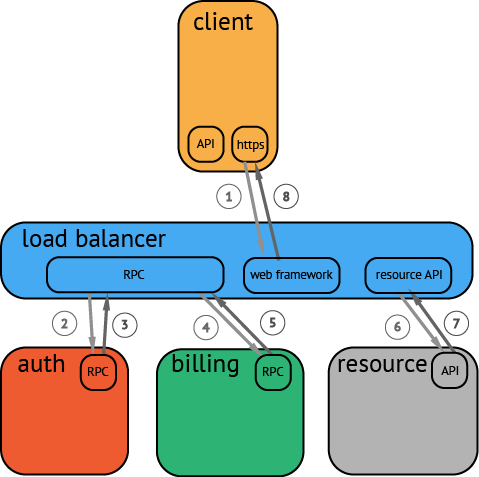
\includegraphics[width=\textwidth,height=6cm,keepaspectratio=true]{basic_trace}
\caption{A sample trace}
\label{basic_trace}
\end{figure}

\begin{figure}
\centering
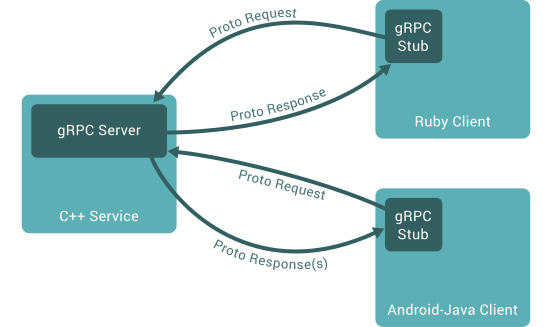
\includegraphics[width=8cm,height=6cm,keepaspectratio=true]{grpc_arch}
\caption{Architecture of gRPC}
\label{grpc_arch}
\end{figure}




\section{Background}
This section will provide an overview on Opentracing, the 
types of wire protocols that we explore for cross-process communication
and how annotations are propagated through them, and the reasoning behind 
integrating the fault injection mechanism into the tracing framework.


\subsection{OpenTracing}
Today's microservice architectures are large in scale and highly complex, often consisting 
of services written many languages; this makes distributed tracing over these services
extremely challenging. Opentracing\cite{opentracing:doc} provides a set of vendor-neutral
APIs for obtaining distributed traces through annotation propagation and allows for an easy
integration into existing microservice architectures. Previous solutions for tracing through
application level annotations such as Magpie\cite{magpie} and X-Trace\cite{xtrace} are unappealing
because of the per-application schema requirement and high overhead\cite{sigelman:dapper}. For these reasons,
we chose to use the Opentracing APIs to provide our architecture with fine-grained traces. 



\subsubsection{Trace Terminologies}
A \textbf{Span} is a basic, logical unit of work with a start time and duration, and exists within 
a single service; spans can be nested to show causal relation. A \textbf{Baggage} is a set of \textless K,V\textgreater pairs wrapped within a span's context, and allows for transparent propagation of arbitrary data. A \textbf{Tracer} consists of a set of Spans that belongs to a group of services; for example: a set of REST endpoints belonging to a group of services in a server. For cross-process tracing, a tracer will \textbf{inject} the span's context, and \textbf{extract} it on the other end.



\subsubsection{Trace flow}
Each service that a developer wishes to be traced will need to have a span constructed, after which it
will be added to a list of spans in the global tracer. Each span will automatically provide trace detail consisting of a timestamp and duration; the developer can decorate the span with more details, such as the status of a lock or value of a variable by adding to the span's baggage. When a service calls another service,
the tracer will have to be invoked to inject the local span's context into the wire, and extracted on the other side. During the extraction, a new(child) span is constructed from old(parent) span's context. Spans are recorded in the order that they are finished, meaning that whichever finishes first will be first to output trace information to the output stream. Figure \ref{basic_trace} shows a simple trace involving several microservices\cite{opentracing:doc}.


\subsection{Fault Handling}
There are three ways one could approach adding a fault injection component into a service consisting of
microservices, each of which have its own advantages and disadvantages over the other. The first way to approach this problem is to add the component in the services themselves, and each service will have its own chunk of code that will react accordingly as it receives information from upstream. The obvious advantage to this approach is that it is easy to implement and the developer has full control on how each service should react to a type of failure. However, this would mean that the code would have to be present in all the services, which could be a daunting task if there are tens if not hundreds of services written in a multitude of languages.

The second approach would be to have the wire protocol handle the fault itself. If all of the services are communicating through a single protocol, say HTTP, then this would greatly reduce the amount of coding that needs to be done in order to trigger faults. Even if the subsets of the services use different protocols, the amount implementation that needs to be done is proportional to the number of protocols used, which should be in the single digit. The downside to this approach would be the need to add an extension to the protocol, maybe even modifying core components in the protocol itself which could lead to bugs that might possibly violate the protocol's integrity.

The third approach would be to provide fault handling per programming language. This is the approach that we have chosen in our implementation, which will be provided in detail later on. This implementation is manageable in a sense that the number of languages in a service is bounded between ten and twenty, and we avoid the risk of polluting our code or the code of the wire protocol that we use. As an example, suppose we have a set of HTTP REST endpoints which are written in golang\cite{google:golang}, the only changes we need to make are to wrap our handler functions inside a decorator. Below is a code listing of how one would implement this:


\begin{lstlisting}[
    basicstyle=\tiny, %or \small or \footnotesize etc.
]

func homeHandler(w http.ResponseWriter, r *http.Request) {
    //stuff goes here
}

func decorate(f http.HandlerFunc) http.HandlerFunc {
    return func(w http.ResponseWriter, r *http.Request) {
        //do some preprocessing of the request
        f(w, r) //call the function
    }
}

func main() {
    http.HandleFunc("/home", decorate(homeHandler))

    http.ListenAndServe("localhost:8080", nil)
}
\end{lstlisting}

Notice that the changes to the application are minor, and that the decorator has full access to whatever was passed over the wire.



\subsection{Wire Protocols}
Wire protocols are used for writing application level code for cross-process communication. 
Protocols such as HTTP, gRPC\cite{google:grpc}, Thrift\cite{apache:thrift} provides a way for
services to receive data as they are called. Opentracing supports both HTTP and gRPC as wire protocols,
and uses them as a mean to propagate span context. In gRPC, clients specify methods that can be called 
remotely which the server will implement and handle client calls, and data is passed along gRPC wire in the 
form of Protocol Buffers\cite{google:protobuf}. The basic flow of the gRPC architecture\cite{google:grpc} can be seen in Figure \ref{grpc_arch}.



\subsection{Why integrate FI and tracing?}
We believe that fine-grained traces and request-level fault injection are complementary to one another.
One of the reasons we seek detailed traces in large scale, distributed services is to analyze a result
of a bad execution to find weak points that prevented a response to the client's request. It is on these
same weak points that we would like to inject faults to verify the failure in order for developers to fix.
Since Opentracing already provides a mean to easily pass arbitrary baggage between services, we would like
to take advantage of this and propagate request-level faults through baggage items. Of course, one could propagate such requests through the wire protocols themselves, bypassing the overhead of constructing spans and injecting them; however, the overhead of construction and injection are extremely small, and Opentracing's APIs allow for a clean way of handling the baggage data. 


\begin{figure}
\centering
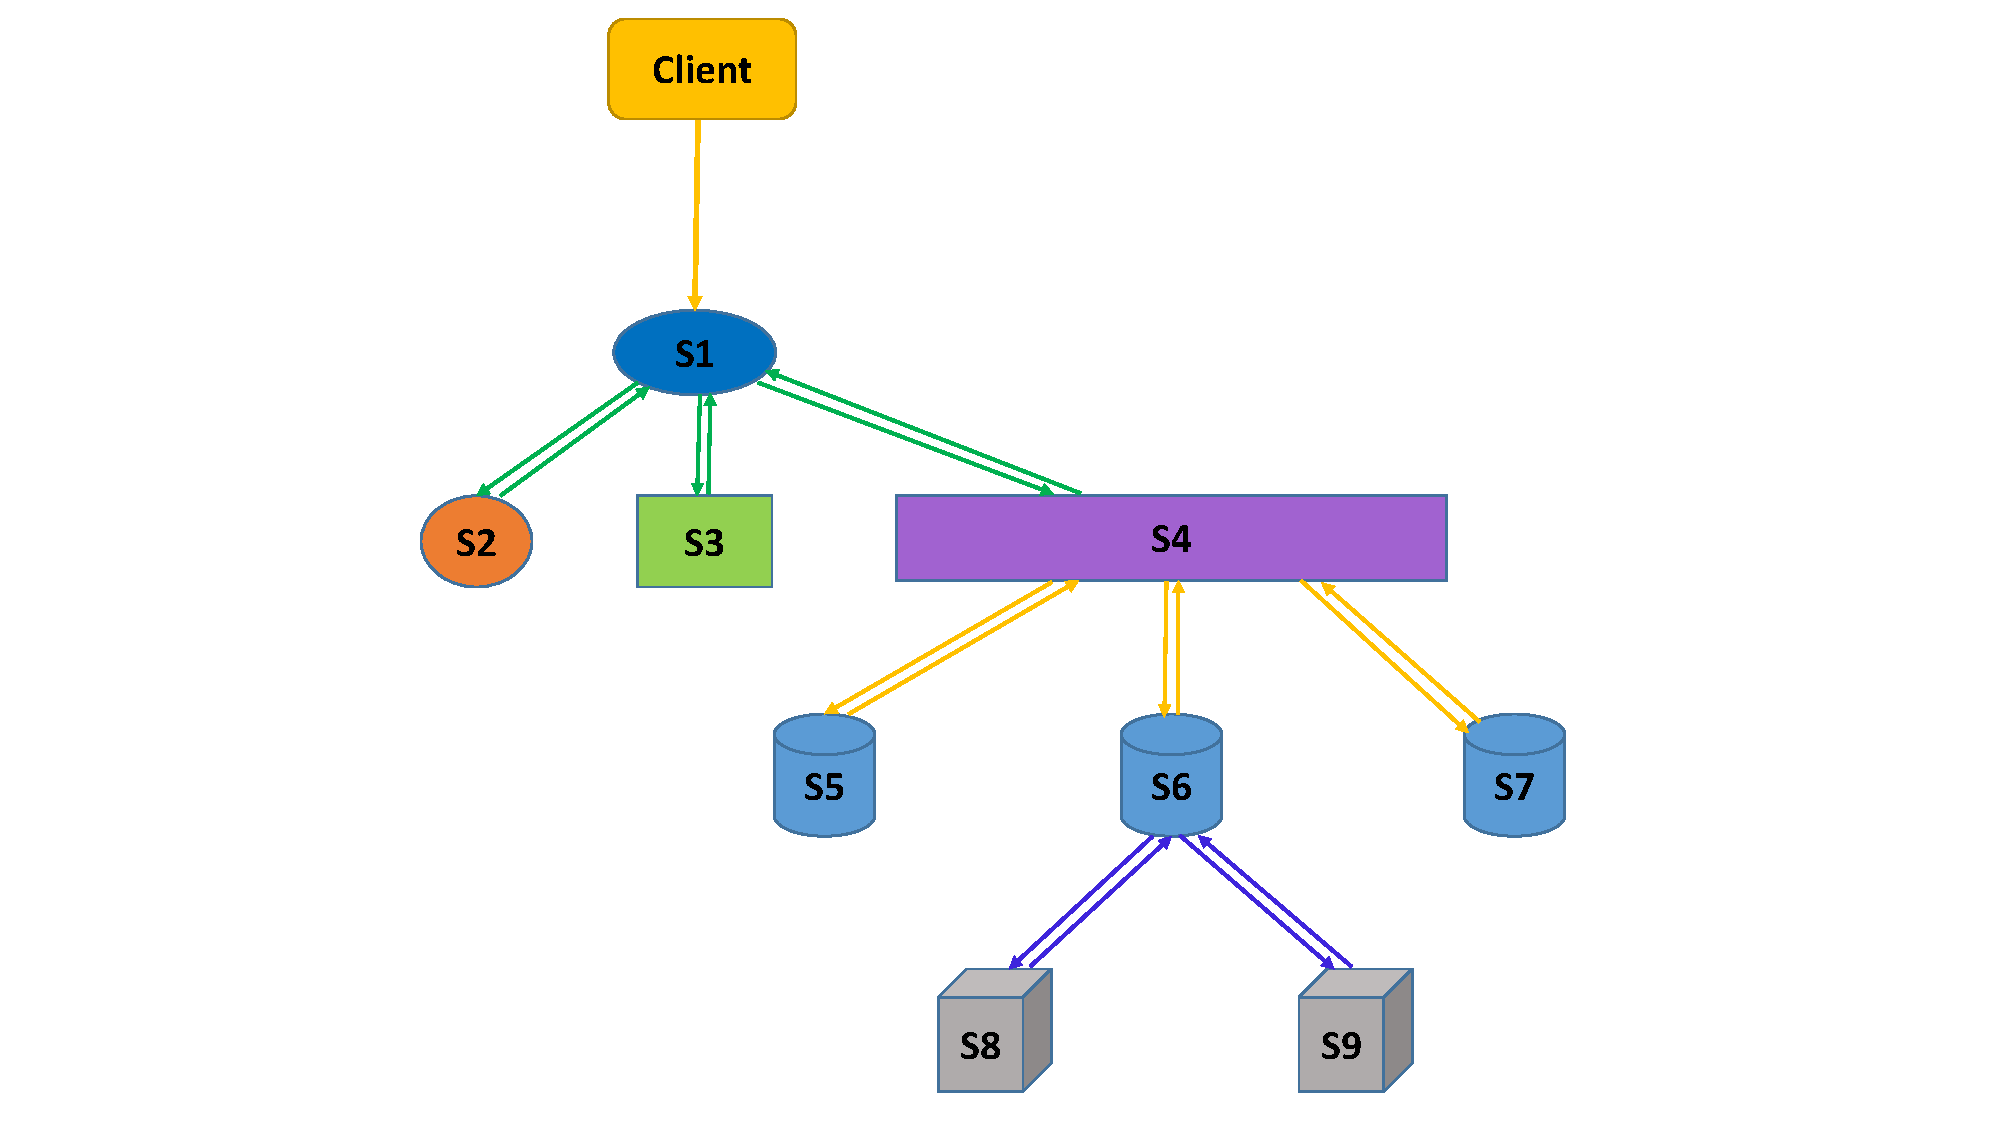
\includegraphics[width=8cm,height=10cm,keepaspectratio=true]{toy_architecture}
\caption{Test architecture consisting of a small set of microservices}
\label{toy_arch}
\end{figure}


\section{Implementation} \label{implementation}
This section details the implementation choices that we have chosen to pursue to build our framework. Because we do not have a real microservice architecture to perform tests on, we built a simple service consisting of two \textbf{servers} listening on two different ports and a set of services contained in each server, the architecture of which can be seen in Figure \ref{toy_arch}. The services are coded to construct spans upon being called, and will provide detailed traces of their states. The \textbf{client} will start by invoking service1 on the first server, which will trigger the full call graph and provide the complete trace.

We chose \textbf{golang}\cite{google:golang} as our programming language because of its extensive support for the Opentracing framework and because of the strength of its \textbf{decorator} syntax. In total, the lines of code is just shy of 500 lines including the code for the servers, client, and the fault handling mechanism. The wire protocol chosen was \textbf{HTTP} in the form of REST method calls, and support provided by Golang made it very easy to integrate a decorator that wraps around all of the services. 

We leverage the powerful \textbf{Baggage} annotation provided by Opentracing to propagate our failures downstream. The client can accept as argument any service that it wants to target for failure testing, and will inject a baggage item whose key serves as a flag into its own span. This baggage is then propagated to whichever service that it calls, and further downstream if the said service calls upon other services all of which can see the client span's baggage items. Because we have decorated our handler to intercept service calls, our decorator will detect if the failure flag exists before proceeding to calling the service itself. If the flag exists, and the decorator notices that the service at hand matches that which has been signaled for failure, then it will act and perform the injection. 

Two of the most common types of failures in distributed services are \textit{unknown delays} and \textit{packet lost}. When services send data to one another, we can never be certain when, or if, the data will arrive. In our implementation, we allow the tester to specify the delay time to see how the upstream services react, and the decorator will simply sleep for this duration before calling the service itself. To simulate packet lost, we have the decorator ignore the request and never actually call the service. 

The verification step to see if our fault injection does work as intended is fairly straightforward. To verify that a delay is actually injected, we simply check that a service's span traces will be delayed for said period of time before being printed. To verify that a packet has indeed been dropped, we check that the service's span traces is not printed along with the other spans' traces.


\begin{figure}
\centering
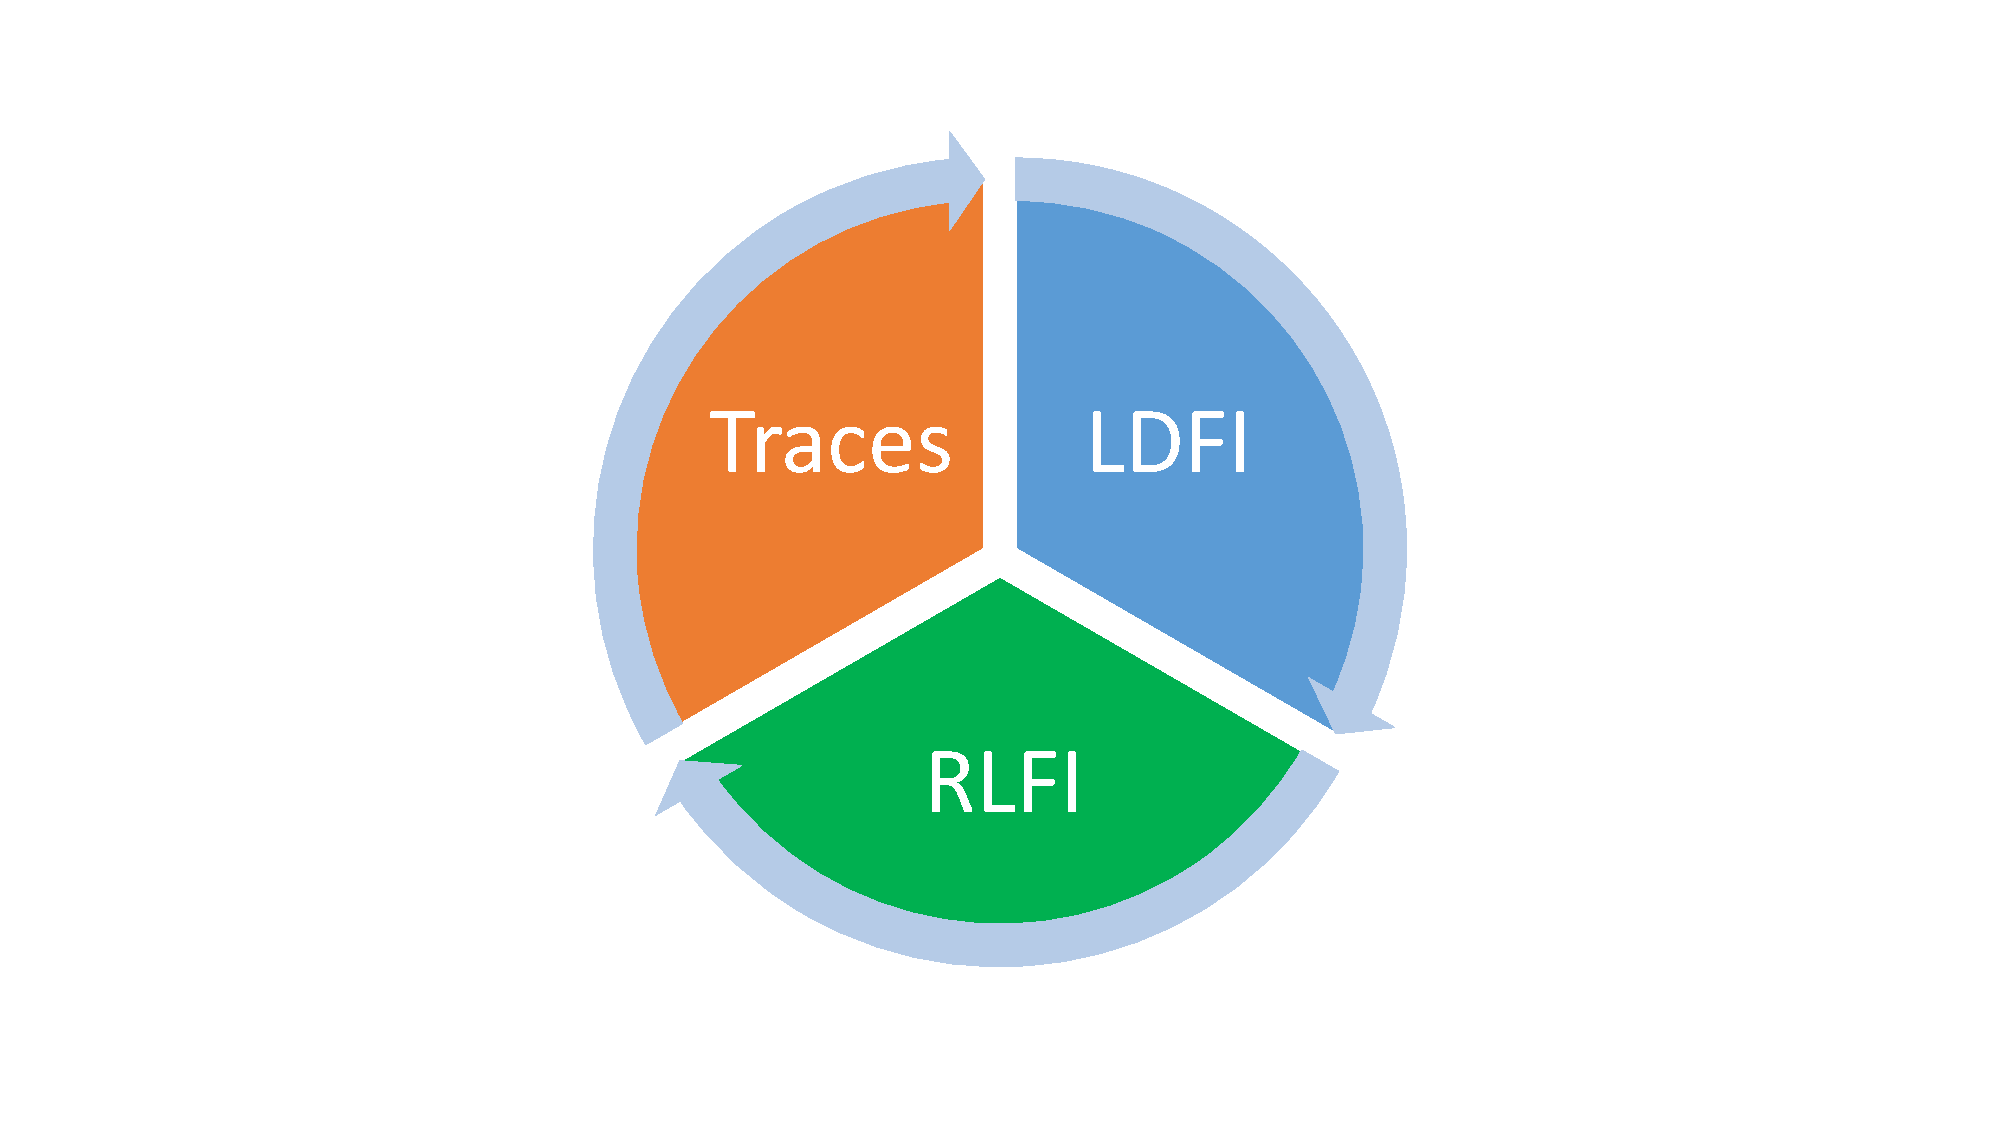
\includegraphics[width=8cm,height=10cm,keepaspectratio=true]{puzzle}
\caption{Fine-grained tracing, LDFI and RLFI completing the puzzle of debugging distributed systems}
\label{puzzle}
\end{figure}

\section{Future Work}
The current implementation of RLFI is but a proof-of-concept to show that we can perform fault injection experiments efficiently in a controlled setting, and obtain fine-grained traces to understand how the system reacts to such faults. Our current focus is to extend the implementation so that it supports a multitude of languages, not just Golang. While there is still much work to be done with RLFI, it is but one piece of a puzzle to understand and debug behavior of complex distributed systems, as shown in Figure\ref{puzzle}.

It is next to impossible to obtain a real life service from industry partners to perform our tests on, mainly because our partners do not want to risk their services being rendered useless or confidential information such as software architecture and personal client information to be exposed. Also, when compared to the real world, our toy architecture is but a measly branch in a huge tree of microservices. We hope to integrate our tracing and fault injection framework into a microservice generator which would generate graphs of size in resemblance of ones found in industry; this generator is undergoing development by a team member in our lab.

To manually dig through traces to find interesting points of failure for RLFI is a daunting task to say the least. Molly, an implementation of Lineage Driven Fault Injection, is a tool developed by Peter Alvaro et al.\cite{alvaro:ldfi} that is perfectly suited for our situation. We can feed the good traces that our system produces into LDFI, which will find the critical points of failure in our system. With the critical points found, we carefully inject the faults into the system and determine whether the fault handling mechanism of the service will is sufficient. We continue this cycle of tracing, reasoning, and injecting failure until we have a system that is robust enough for us to sleep soundly at night.

Currently the traces that results from our framework are cluttered and requires parsing to make it more human readable. We would like to develop a small, offline tool that will parse the traces into something that LDFI can understand and also produce a visual call graph for ease of verification. 


\section{Related Work}
Previous work on fault injection such as the Netflix Simian Army\cite{netflix:chaosmonkey} provides a set of tools for inducing faults such as randomly crashing processes have been released on their webservice running on Amazon's cloud. The downside to randomly crashing nodes is the cost of restarting the nodes again, which RLFI avoids. Orchestra\cite{orchestra}, a fault injection environment developed by Scott Dawson et al. requires changes to the raw socket API, which might seem appealing to those who prefer application level instrumentation. Ferrari\cite{ferrari} is similar to how RLFI current introduce faults in that it relies on software traps that are triggered by events such as memory access to actually inject the faults.

Magpie\cite{magpie} is a modeling service that collects request-level traces across a distributed system, but requires that applications follow a specific schema. X-trace\cite{xtrace} also provides fine-grained traces through an annotation propagation scheme, but the performance is greatly impacted because of the abundace in metadata recorded. Zipkin\cite{zipkin} requires application level implementation of the client and server, and contains components that are not useful for our aim. Dapper\cite{sigelman:dapper} greatly resembles the Opentracing architecture, but it is internally deployed at Google. 


\section{Conclusions}
Intelligent failure testing in modern microservice architectures plays an important part in preventing rare bugs from causing headaches to developers and keeping services available to clients. Previous approaches to failure injection are either missing important combinations of failure due to the randomness involved, or require modifications to the low-level communication interface. RLFI works by propagating failure flags through \textit{baggage} annotations provided by Opentracing\cite{opentracing:doc}, and handle faults by wrapping a decorator around the wire protocol's handler function as described in section \ref{implementation}. 

In addition to fault injection at the request level, RLFI is integrated with a tracing framework that will provide fine-grained traces of the underlying system both before and after the injection experiment. Through Opentracing, we can piggyback failure flags over the wire, and visually verify system response from the resulting traces. RLFI with tracing and LDFI\cite{alvaro:ldfi} allows us to complete the puzzle of debugging distributed systems.


\section{Acknowledgments}
We would like to thank Peter Alvaro for the initial suggestion to explore Opentracing for fault injection which materialized this project, and the extremely helpful feedback on both design and implementation of the framework. We also thank Nikhil Kini and Kamala Ramasubramanian for the helpful feedback provided as this project was presented, and we thank Ashutosh Raina, Kathryn Dahlgren, Sarah Borland and Asha Karim for making use of the traces for their projects. Last but not least, we thank the team at Netflix and Lightbend for making us realize that our work is very much relevant to their every day need in the industry setting.

\bibliographystyle{acm}
\bibliography{sample}

\end{document}







